\documentclass{beamer}
\usetheme{CambridgeUS}
\usefonttheme[onlymath]{serif}
\title{Aiyagari model in niqlow}
\author{Nam Phan}
\date{\today}
\usepackage{geometry}
\usepackage{graphicx}
\usepackage{caption}
\usepackage{amsmath}
\usepackage{upgreek}
\usepackage{amssymb}
\usepackage{physics}
\usepackage{accents}
\usepackage{bbold}
\usepackage{bm}
\newcommand{\ubar}[1]{\underaccent{\bar}{#1}}

\begin{document}
	
	\begin{frame}
		\titlepage
	\end{frame}

\begin{frame}
\frametitle{Outline}
\tableofcontents
\end{frame}


\section{Brief introduction}

\begin{frame}
\frametitle{Introduction}
\begin{itemize}
	\item Aiyagari (1994) or Bewley-Huggett-Aiyagari (BHA) is a workhorse model to study economy with heterogeneous agents in a general equilibrium setup
	\begin{itemize}
		\item Application: Precautionary saving, liquidity constraints, distribution of wealth and income.  
		\item Extension: Macro labour (health, education). Fiscal policy (gov transfer, taxation)
		\end{itemize}
	\item Key assumption:
	\begin{itemize}
		\item Agents face uninsureable idiosyncratic shock and markets are incomplete 
	\end{itemize}
\end{itemize}

\end{frame}

\AtBeginSection[]
{
\begin{frame}
\frametitle{Outline}
\tableofcontents[currentsection]
\end{frame}
}


\section{Model}

\begin{frame}
\frametitle{Model}
Model details:
\begin{itemize}
	\item Infinite horizon (extension: finite life-cycle)
	\item Single asset (extension: multiple assets)
	\item Inelastic labour supply (extension: endogenous labour choice)
	\item Agents face idiosyncratic labour shocks (extension: aggregate shock, or with both)
	\item Closed economy (extension: open economy yet)
	\item Representative firm (extension: heterogeneous firms)
	\item No government, no central bank (extension: with either or both)
	\item Walrasian labour and good market (extension: decentralized search market)
\end{itemize}
\end{frame}


\begin{frame}
\frametitle{Household} 
Solves the following infinite horizon problem: 
\begin{equation}
\begin{aligned}
& \max E_0 \bigg[ 
\sum_{t=0}^{\infty} \beta^t U(c_t )	\bigg] \\
 \text{s.t: } 
& c_t + a_{t+1} = a_t (1 + r_t)  + w_t \epsilon_t \\ 
& a_{t+1} \geq \ubar{a} \\ 
\end{aligned}
\end{equation}
where $\epsilon_t \in \mathcal{E}$ is labour shocks. Assume that labour shock is AR(1) process in logs: 
\begin{equation}
\begin{aligned}
\epsilon_t^i = \exp(z_t^i) \\ 
z_t^i = \rho z_{t+1}^i + v_t^i \\ 
v \sim N(0,\sigma_v^2)
\end{aligned}
\end{equation}
\end{frame}





\begin{frame}
\frametitle{Household}
\begin{itemize}

\item Focus on steady-state equilibrium where $r_t = r, w_t = w, \forall t=0,1...$. Bellman equation for the problem above is: 

\begin{equation}
\begin{aligned}
V(a,\epsilon) 
& = \underset{a',c}{\max } 
\bigg\{ U(c) 
	+ \beta \sum_{\epsilon' \in \mathcal{E} } \Pi(\epsilon'|\epsilon) V(a',\epsilon) 
		\bigg\} \\ 
\text{s.t: } 
& c + a' = a(1+r) - w \epsilon  \\ 
& a' \geq \ubar{a} \\ 
\end{aligned}
\end{equation}
where $\Pi(\epsilon'|\epsilon)$ describes the transition of labour shock. \\  

\item Solving the Bellman equation gives the policy function $a'(a,\epsilon),c(a,\epsilon)$ and value function $V(a,\epsilon)$. 
\end{itemize}
\end{frame}


\begin{frame}
\frametitle{Distribution over state-space} 
\begin{itemize}
	\item Construct a probability density function $\lambda(a,\epsilon)$ over state-space, and a transition matrix 
	$Q\big( (a',\epsilon'), (a,\epsilon) \big)$
	\item $\lambda(a,\epsilon)$ returns the proportion of population with asset $a$ and current labour productivity state $\epsilon$. Thus heterogeneous agent model. 
	\item Agents face different labour shock profile, thus heterogeneous in asset accumulation. 
	\begin{itemize}
		\item Uninsured idiosyncratic risk is the key 
	\end{itemize}
\end{itemize}
\end{frame}




\begin{frame}
\frametitle{Distribution over state-space} 
The distribution $\lambda$ evolves according to the following Markov chain: 
\begin{equation}
\begin{aligned}
\lambda_{t+1}(a_{t+1},\epsilon_{t+1}) 
= 
\sum_{a_{t} \in \mathcal{A}} 
\sum_{\epsilon_{t} \in \mathcal{E}} 
Q\big( (a_{t+1},\epsilon_{t+1}),(a_t,\epsilon_t) \big)
\lambda_{t}(a_t,\epsilon_t)
\end{aligned}
\end{equation}
where $\mathcal{A} = [\ubar{a},\infty) $ is the action space, and: 
\begin{equation}
\begin{aligned}
Q\big( (a_{t+1},\epsilon_{t+1}),(a_t,\epsilon_t) \big) 
= \bm{1} \big( a_{t+1} = a'(a_t,\epsilon_t)  \big) \Pi(\epsilon_{t+1}|\epsilon_t) 
\end{aligned}
\end{equation}
Stationary distribution satisfies: 
\begin{equation}
\begin{aligned}
\lambda_{t+1} = \lambda_t
\end{aligned}
\end{equation}
or equivalently
\begin{equation}
\begin{aligned}
\lambda^* = \lambda^* Q
\end{aligned}
\end{equation}
Note that $\lambda^*$ is an equilibrium object. 

\end{frame}


\begin{frame}
\frametitle{Firm} 
A representative firms solves the following (static) profit maximization problem: 
\begin{equation}
\begin{aligned}
\max AF(K_t,H_t) - w_t H_t - r_t K_t - \delta K_t
\end{aligned}
\end{equation}
where $A$ is an aggregate productivity level. In a stationary equilibrium, FOC gives: 
\begin{equation}
\begin{aligned}
w = A F_H(K,H) \\ 
r + \delta = A F_K(K,H)
\end{aligned}
\end{equation}
\end{frame}





\begin{frame}
\frametitle{Market clearing}
\begin{enumerate}
	\item Good: 
\begin{equation}
\begin{aligned}
\sum_{a \in \mathcal{A}} 
\sum_{\epsilon \in \mathcal{E}}
c(a,\epsilon) \lambda(a,\epsilon)
+
\sum_{a \in \mathcal{A}} 
\sum_{\epsilon \in \mathcal{E}}
a'(a,\epsilon) \lambda(a,\epsilon)
= AF(K,H) - \delta K
\end{aligned}
\end{equation}
\item Labour: 
\begin{equation}
\begin{aligned}
H 
= 
\sum_{a \in \mathcal{A}} 
\sum_{\epsilon \in \mathcal{E}}
\epsilon \lambda(a,\epsilon)
\end{aligned}
\end{equation}
\item Capital: 
\begin{equation}
\begin{aligned}
K
=
\sum_{a \in \mathcal{A}} 
\sum_{\epsilon \in \mathcal{E}}
a'(a,\epsilon) \lambda(a,\epsilon)
\end{aligned}
\end{equation}
\end{enumerate}
\end{frame}



\begin{frame}
\frametitle{Stationary Recursive equilibrium (RCE)} 
RCE is a value function $V(a,\epsilon)$, and policy functions $c(a,\epsilon)$ and $a'(a,\epsilon)$; firm's decision for aggregate factor demand $K$ and $H$; prices $w$ and $r$; and a stationary measure $\lambda^*$ such that: 
\begin{itemize}
	\item Given $r$ and $w$, policy functions $c$ and $a'$ solve the household's problem, and $V$ is the associated value function
	\item Given $r$ and $w$, aggregate factor $K$ and $H$ solves the firm's profit maximization problem 
	\item Markets for good, labour and capital clear
	\item Stationary measure: 
\begin{equation}
\begin{aligned}
\lambda^*(a,\epsilon) 
= \sum_{a \in \mathcal{A} } 
\sum_{\epsilon \in \mathcal{E}} 
Q\big( (a',\epsilon'),(a,\epsilon) \big)
\lambda^*(a,\epsilon)
\end{aligned}
\end{equation}
\end{itemize}

\end{frame}


\section{Algorithm}
\begin{frame}
\frametitle{Algorithm}
Nested fixed loop algorithm: 
\begin{itemize}
	\item For given prices $\hat{r}$ and $\hat{w}$, solve for an inner loop:
	\begin{itemize}
		\item Solve for value function and policy function
		\item Initialize an agent measure $\lambda(a,\epsilon)$ and construct transition matrix $Q$. 
		\item Iterate $\lambda_{t+1} = \lambda_t Q$ until convergence. Obtain stationary measure $\lambda^*$
	\end{itemize}
\item Outer loop: 
\begin{itemize}
	\item Compute aggregate factor $K$ and $H$ implied by policy function and agent measure $\lambda^*$. 
	\item Compute prices $r$ and $w$ implied by firm's FOCs (market clearing prices)
	\item If $r$ and $w$ are different than $\hat{r}$ and $\bar{w}$, update prices and go back to the inner loop. 
\end{itemize}
\end{itemize}
\end{frame}

\begin{frame}
\frametitle{Model result}
\begin{center}
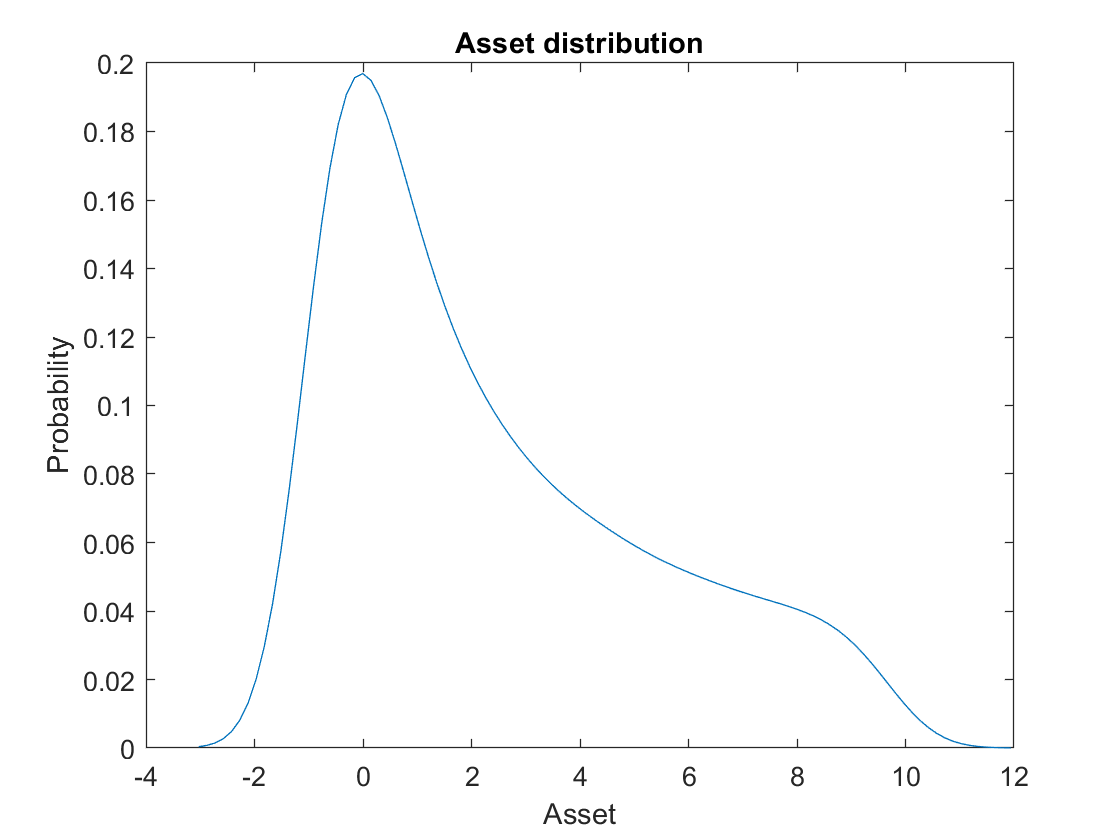
\includegraphics[scale=0.3]{graph.png} \\
Kernel plot of $a'(a,\epsilon)$ for $\mathcal{A} \in [-1,10]$
\end{center}
\end{frame}

\begin{frame}
Few notes: 
\begin{itemize}
	\item In theory, $\mathcal{A} = [\ubar{a},\infty)$. In practice, we normally discretize the state-space and experiment with the upper bound $\bar{a}$
	\item Value function can be solved by Value function iteration or Policy function iteration. 
	\item Equilibrium prices could be found bi-section method. 
\end{itemize}
\end{frame}

\section{Aiyagari in niqlow}
\begin{frame}
\frametitle{Summary for niqlow input}
\begin{itemize}
	\item Clock: Ergodic
	\item Action variable: $a'(\theta) \in \mathcal{A} = [\ubar{a},\bar{a}]$
	\item States: $\theta = (a,\epsilon)$
	\item Transition: 
	\begin{equation}
	\begin{aligned}
	& a' = a(1+r) - w \epsilon - c \\ 
	& \log(\epsilon') = \rho \log(\epsilon) + v, v \sim N(0,\sigma_v^2)
	\end{aligned}
	\end{equation}
	\item Utility: 
	\begin{equation}
	\begin{aligned}
	U(c) = \dfrac{c^{1-\sigma}-1 }{1-\sigma}, \sigma > 0
	\end{aligned}
	\end{equation}
	\item Stationary distribution: 
	\begin{equation}
	\begin{aligned}
	\lambda^*(a,\epsilon) 
	= \sum_{a \in \mathcal{A} } 
	\sum_{\epsilon \in \mathcal{E}} 
	Q\big( (a',\epsilon'),(a,\epsilon) \big)
	\lambda^*(a,\epsilon)
	\end{aligned}
	\end{equation}
\item How about solve for equilibrium prices $w$ and $r$? 
\end{itemize}

\end{frame}









\end{document}